\documentclass[12pt]{article}
\usepackage{amsmath}
\usepackage{graphicx}
\usepackage{hyperref}
\usepackage[latin1]{inputenc}
\usepackage[margin=.5in]{geometry}


\title{Problem Set 3}
\author{\vspace{-2.0cm}Joanne Wardell}
\date{9 May 2019}

\begin{document}
\maketitle

\begin{figure}[!h]
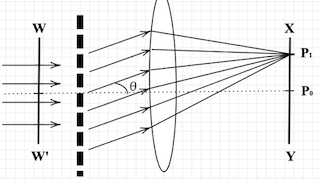
\includegraphics{pic1.png}
\end{figure}

Take a grating with $N$ slits. The let $e$ be the slit width and $d$ be the width of the opaque material between consecutive slits. Monochromatic light with a wavelength $\lambda$ is shone through the grating. The slits cause each light ray to create secondary wavelets in all directions. The wavelet which doesn't deviate from its indicent path arrives at point $P_{0}$, but take a ray which deviates from its indicent path by $\theta$. The secondary wavelets enter a lens and encounter a phase change as well as a refraction, reaching point $P_{1}$, creating diffraction and fringe patterns with varying intensity.

Approximate the secondary wavelets at each slit as a single wave with amplitude $A\frac{\sin{\alpha}}{\alpha}$ where $\alpha = \frac{\pi}{\lambda}e\sin{\theta}$. Since there are $N$ slits, there are $N$ of these. The path difference between two slits is $e + d$ so the phase difference is $\delta = \frac{2\pi}{\lambda}(e+d)\sin{\theta}$. We'll call this $2\beta$. Making use of the angle of deviation formula for the resultant ampltude $a\frac{\sin{\frac{1}{2}(\alpha + \delta)}}{\sin{\frac{\alpha}{2}}}$ the amplitude at $P_{1}$ is \\
\[\frac{A\sin{\alpha}}{\alpha}\cdot\frac{\sin{N \beta}}{\beta}\]
and using Malus's law the intensity is 
\[I = \frac{A^{2}\sin^{2}{\alpha}}{\alpha^{2}}\cdot\frac{\sin^{2}{N \beta}}{\beta^{2}}\]

Take the derivative of the intensity function and set it equal to zero to find the maxima.

\[\frac{dI}{d\beta} = 2(A\frac{\sin{\alpha}}{\alpha})^{2}\frac{\sin{N\beta}}{\beta}\frac{N\cos{N\beta}\sin{\beta}}{\sin^{2}{\beta}}=0\]
implies
\[N\tan{\beta} = \tan{N\beta}\]

This relationship implies that

\[sin^{2}{N\beta} = \frac{N^{2}}{1 + (N^{2}-1)sin^{2}{\beta}}\]

and so the intensity can be rewritten as

\[I = I_{0}\frac{A^{2}\sin^{2}{\alpha}}{\alpha^{2}}\cdot \frac{N^{2}}{1 + (N^{2}-1)sin^{2}{\beta}}\]

As $N$ becomes larger, the secondary term which governs secondary orders' intensity becomes neglegable, thus

\[I \approx I_{0}\frac{A^{2}\sin^{2}{\alpha}}{\alpha^{2}}\] for the principle maxima.







\end{document}

